\chapter{Problem Description}

The current Bitcoin protocol is depended on the block chain. 
Using a block chain limits Bitcoin in several ways.
These limitations on Bitcoin can be seen as the initial motivation 
for our work to improve the block chain.
But block chain and our improvement can be used in several other fields as well.

Bitcoin and how it uses the block chain technology will be introduced first.
After that the limitations imposed by the block chain will be explained.
Finally an overview will be given of how block chains and our improvements can be used in other fields.

\section{Bitcoin}
\subsection{Block Chain}
For a currency to work, people have to be able to trust that no double spending can occur.%cite
Bitcoin has multiple safe gaurds that work together to prevent double spending.
These safe gaurds will be mentioned during the explanation of how Bitcoin works.

The core of the Bitcoin protocol is the block chain.
The block chain contains every transaction of bitcoins.

A transaction consists of three parts.
The public key of the new owner of the bitcoin,
the hash of combination of the previous transaction together with the public key of the new owner,
and the signature of the hash of the current owner.
The previous transaction is a transaction of the same bitcoin.
The ownership of the bitcoin by the current owner can be verified
by verifying the whole history of the bitcoin.
A transaction is usually shortend to Tx in Bitcoin related work and is used in images in this report.

\begin{figure}[H]
	\centerline{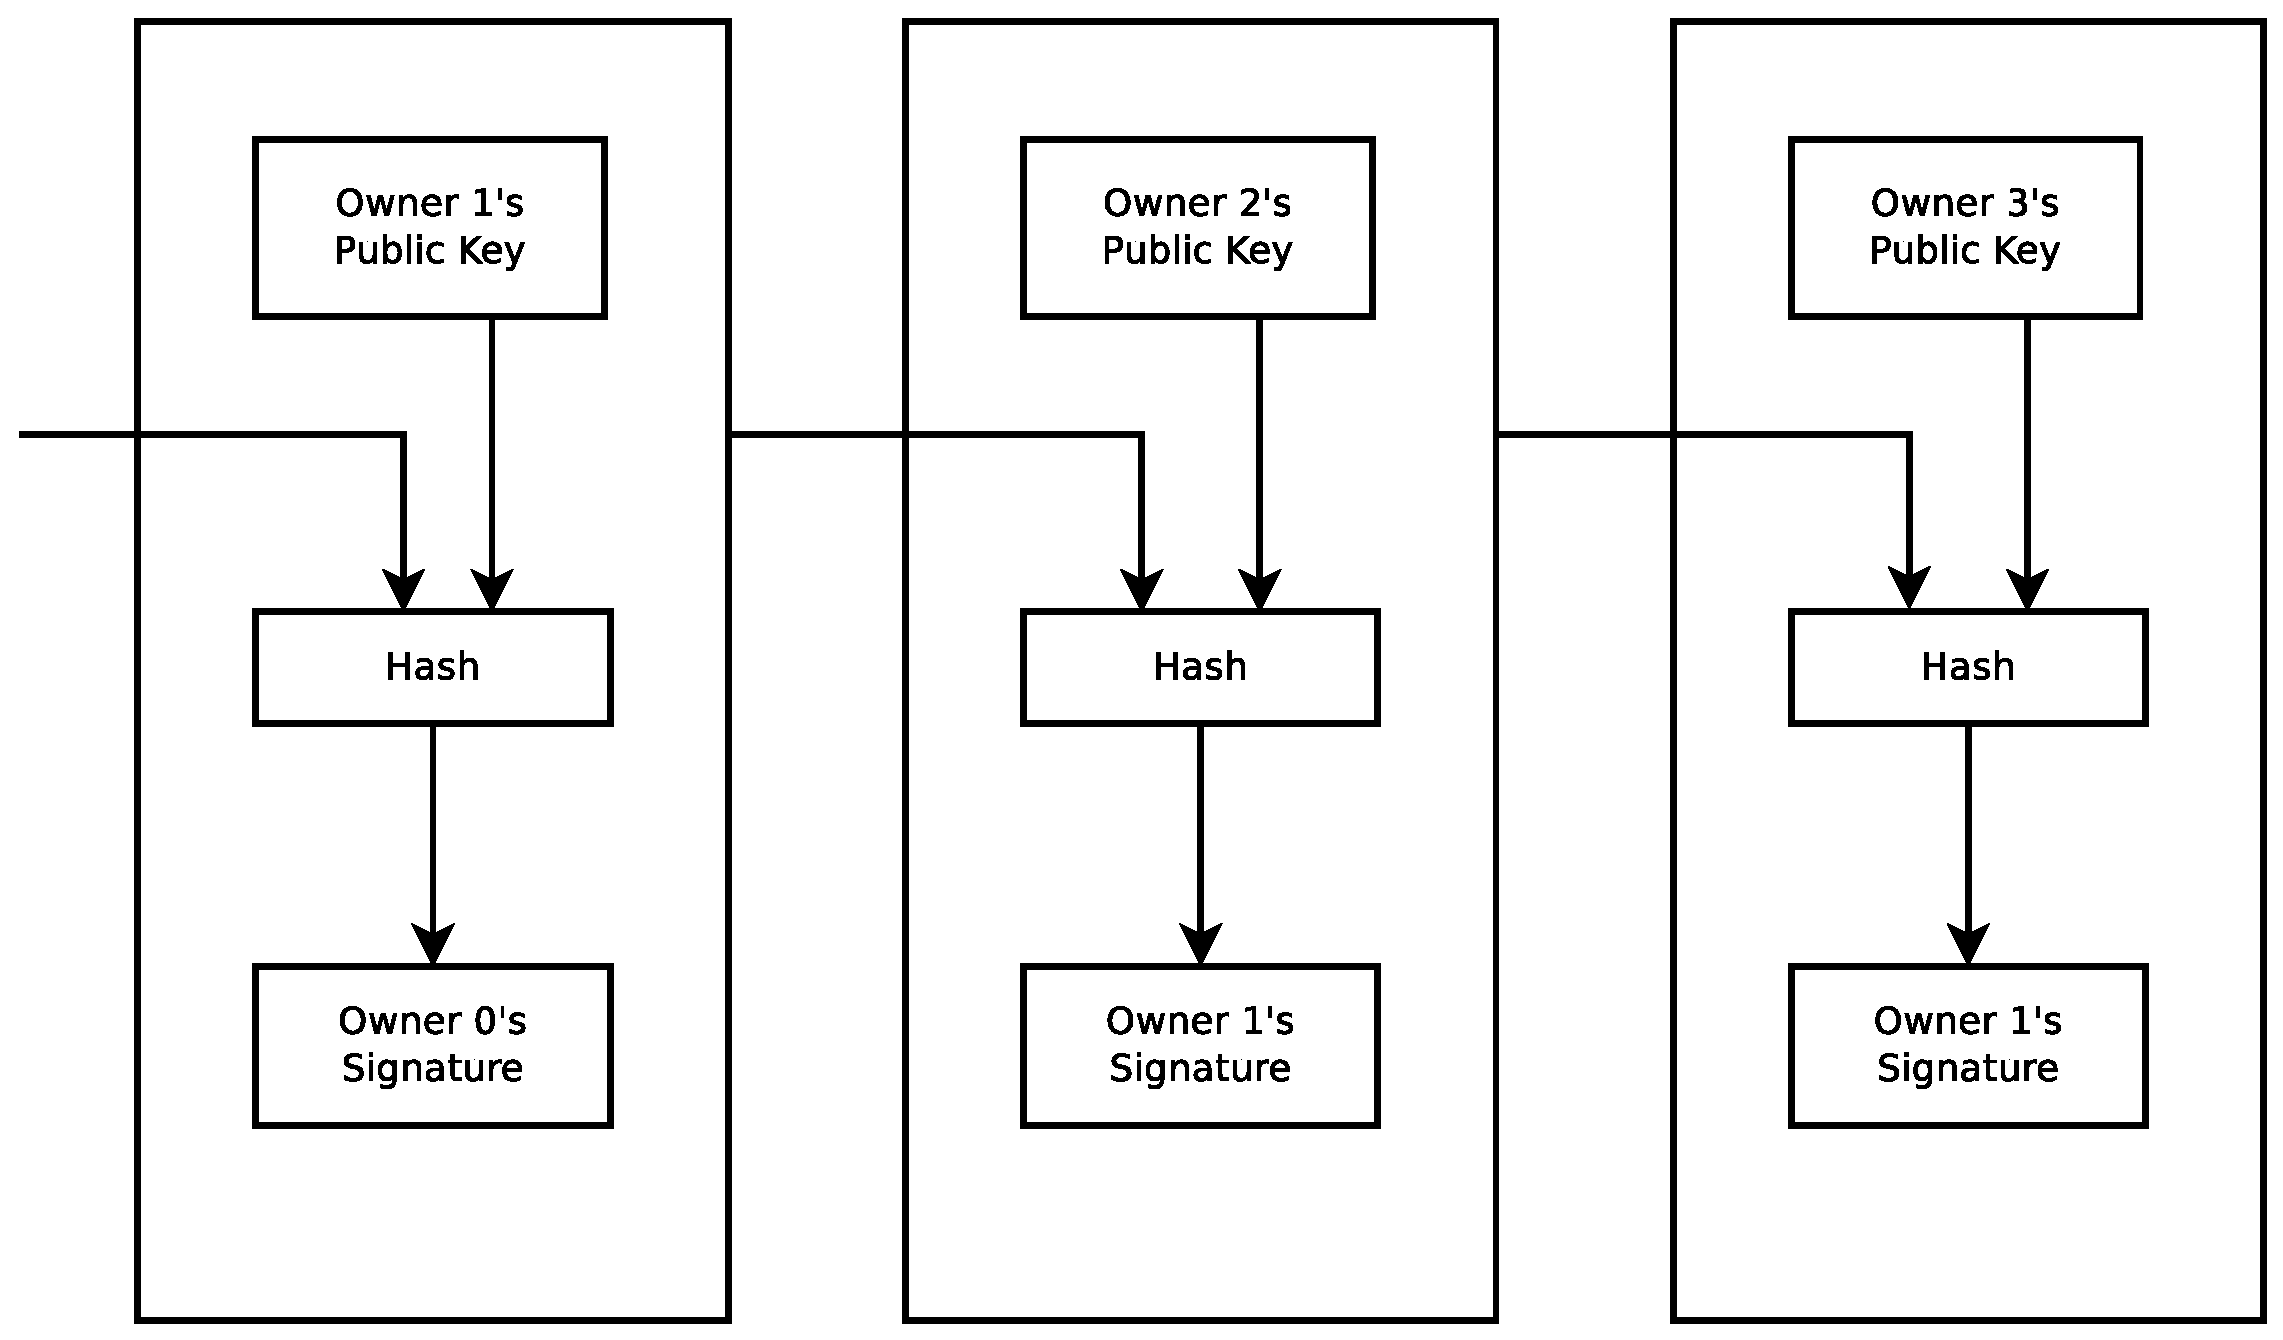
\includegraphics[scale=0.3]{problemDescription/figs/transactions.eps}}
	\caption{Transaction chain}
\end{figure}

Multiple transactions are aggregrated into a single block.
The next block is chained to the previous block by adding the hash of the previous block.
Transaction chains span several blocks inside the block chain.

These blocks are created by nodes in the network, so called miners.
A miner receives transactions from other nodes in the Bitcoin network.
But the transactions are received in a non deterministic way induced by network characteristics.
The non deterministic nature causes blocks to differ from miner to miner.
The order of transactions has to be agreed upon by the network to eliminate this inconsistency.

An attacker can malicously transmit transactions to double spend a bitcoin he owns or does not have.
So every transaction is verified on arrival at a node.
Any transaction that is invalid is just dropped by the node.
No penalty is awarded to the malicous attacker.

Bitcoin uses election based upon Proof-Of-Work system.
A nonce is added to every block. 
This nonce is just a number that can be varied,
but is only sound if the result of the hash of the whole block starts with a certain number of zeros.

\begin{figure}[H]
        \centerline{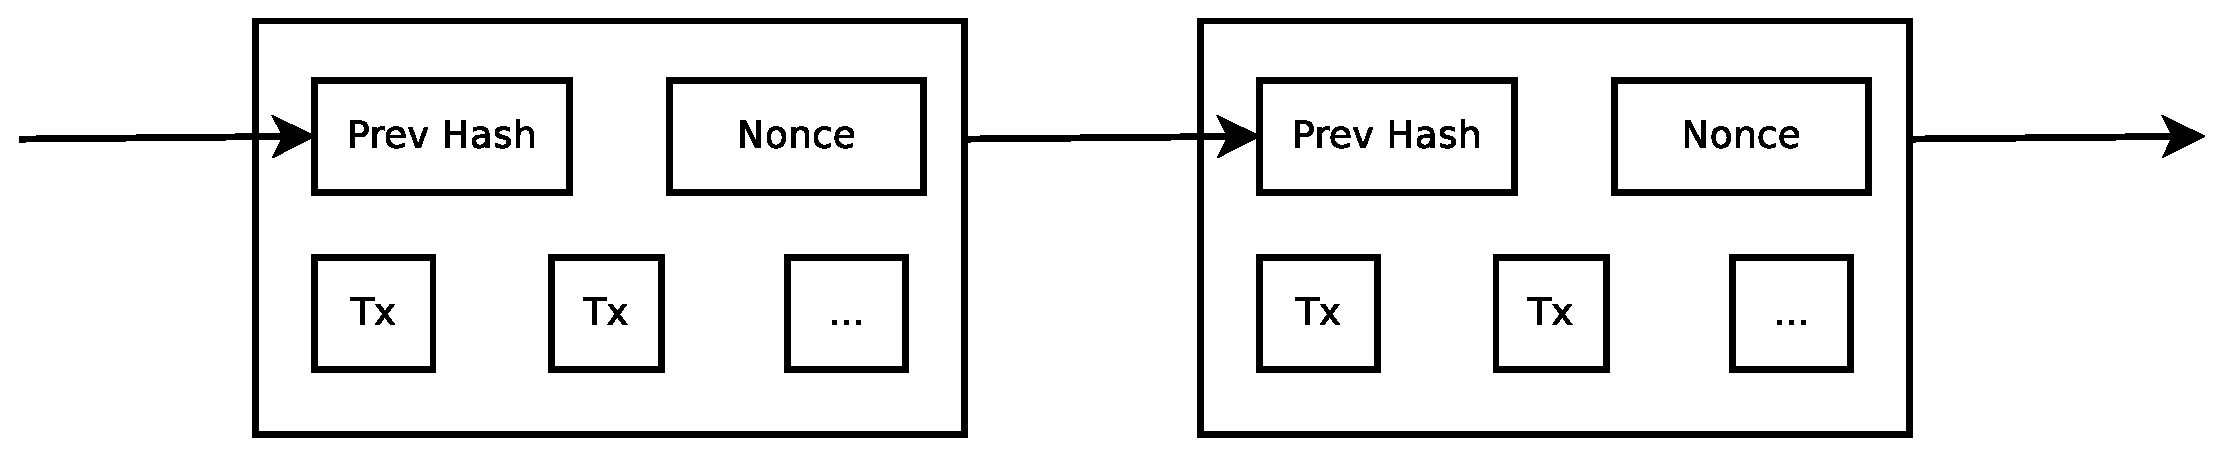
\includegraphics[scale=0.3]{problemDescription/figs/blocks.eps}}
        \caption{Block chain}
\end{figure}

But miners can still find a valid nonce at approximately the same time
and notify parts of the network of their newly found block.
This leaves the network again in an inconsisted state.
These multiple versions of the next block attached to the previous block can be seen as branches.

To solve this inconsistency, Bitcoin nodes save every branch and continue working on the longest branch.
At first the node will favor the first received branch and continue working on that branch
At some point one branch will become predominant in the network
and more nodes will dedicate compute power to extend this branch in comparison to other branches.
Blocks will be found at a faster rate for this branch
and the branch will be adopted by the network as a whole.

The amount of zeros is adjusted to compensate for the increasing speed of being able to find nonces, due to increasing computational power.
The amount of zeros balances the probability of branches occuring
and the time before a new block is found,
which in turn is how fast transactions are processed.

Another way to double spend a bitcoin is by sending a transaction to one part of the network,
but to the other part of the network a transaction with a different receipient.
It can happen that both transactions will at first be processed into a block.
Eventually one branch will one and double spending is averted.

The behaviour just described makes that a transaction can never be confirmed with full certainty.
Another branch could possibly always over take the current longest branch.
This also makes the system susceptible if more compute power is owned by a malicous attacker then honest node, even if it is only 51\%. 
In the end the current branch can be overtaken
and the whole transaction history can be rewritten by the attacker.
Bitcoin introduces points in the chain that are to be considered final and can no longer change.
